\documentclass[a4paper, 12pt]{book}

\usepackage[paperwidth=22.3cm, paperheight=22.3cm, asymmetric, twoside,
bindingoffset=0.76cm, inner=1.27cm, outer=1.27cm, top=1.27cm,
bottom=1.27cm, marginparwidth=0cm,noheadfoot, nomarginpar]{geometry}

\PassOptionsToPackage{unicode}{hyperref}
\IfFileExists{footnotehyper.sty}{\usepackage{footnotehyper}}{\usepackage{footnote}}
\IfFileExists{xurl.sty}{\usepackage{xurl}}{} % add URL line breaks if available
\usepackage{graphicx}
\usepackage{amsmath,amssymb}
\usepackage{longtable,booktabs,array}
\usepackage{calc} % for calculating minipage widths
\usepackage[T1]{fontenc}

\usepackage[dvipsnames]{xcolor}
\usepackage{pagecolor}
\usepackage{anyfontsize}
\usepackage[most]{tcolorbox}
\usepackage[german]{babel}
\usepackage{multicol}
\usepackage{fancyhdr}
\usepackage{wrapfig}
\usepackage{xparse}
\usepackage{listofitems}
\usepackage[symbol*]{footmisc}
\usepackage[colorlinks=true,urlcolor=.,linkcolor=.]{hyperref}
\usepackage{imakeidx}

\makeindex[title={Index}]

% page numbers...
\tcbset{on line,
        boxsep=4pt, left=0pt, right=0pt, top=0pt, bottom=0pt,
        colframe=orange!50, colback=orange, highlight math style={enhanced}}
\fancypagestyle{plain}{
\fancyhf{} % clear all header and footer fields
\fancyfoot[EC,OC]{
\raisebox{\height}{
% \tcbox{\;\textcolor{white}{\thepage}\;}}
 \thepage
}
}
\renewcommand{\headrulewidth}{0pt}
\renewcommand{\footrulewidth}{0pt}}

\pagestyle{plain}

\pagecolor{white}

% fonts...
\usepackage[sfdefault]{roboto}
\usepackage{fontspec}
\setmainfont[Mapping=tex-text]{Roboto}
\setsansfont[Mapping=tex-text]{Roboto}
\setmonofont[Mapping=tex-text, Scale=1]{Courier New Bold}
\newfontfamily\titlefont[Mapping=tex-text]{Roboto}
\newfontfamily\sectiontitlefont[Mapping=tex-text]{Roboto}

\usepackage{amsmath}
\usepackage{unicode-math}
\setmathfont{Fira Math}
\setmathfont[range=up]{Roboto}
\setmathfont[range=it]{Roboto-Italic}
\setmathfont[range=\int]{Fira Math}

% paragraphs...

\parskip5pt
\parindent0pt

% for images...

\ExplSyntaxOn
\NewDocumentCommand{\aspectratio}{smo}
 {% #2 is the image file
  \hbox_set:Nn \l_tmpa_box {\includegraphics{#2}}
  \IfNoValueTF{#3}
   {
    \__student_aspectratio:nn { \box_wd:N \l_tmpa_box } { \box_ht:N \l_tmpa_box }
   }
   {
    \IfBooleanTF{#1}{ \tl_gset:Nx } { \tl_set:Nx } #3
     {
      \__student_aspectratio:nn { \box_wd:N \l_tmpa_box } { \box_ht:N \l_tmpa_box }
     }
   }
 }

\cs_new:Nn \__student_aspectratio:nn
 {
  \fp_eval:n {round( #1 / #2 , 5)}
 }
\ExplSyntaxOff

% templates...

\newsavebox{\storytext}

\newcommand{\PhotoTextC}[3]{ % centered photo+text: image, text, page bgcolor
\savebox{\storytext}{\parbox[b]{\textwidth}{#2}}
\begin{center}
% Compute height (subtract another 20pt to make sure that the text fits, this is hardcoded, FIXME):
\includegraphics[height={\dimexpr\textheight-\ht\storytext-20pt\relax}]{#1}

#2
\end{center}
\pagecolor{#3}
\newpage
\pagecolor{white}
} % \PhotoTextC

\newcommand{\PhotoTextJ}[4]{ % justified photo+text: photo width, image, text, page bgcolor
\begin{center}
 \includegraphics[width=#1\linewidth]{#2}
\end{center}

#3
\pagecolor{#4}
\newpage
\pagecolor{white}
} % \PhotoTextJ

\newcommand{\TextJPhoto}[4]{ % justified text+photo: text, photo width, image, page bgcolor
#1

\begin{center}
 \includegraphics[width=#2\linewidth]{#3}
\end{center}

\pagecolor{#4}
\newpage
\pagecolor{white}
} % \TextJPhoto



\newcommand{\PhotoTextJPhoto}[6]{ % justified photo+text+photo: photo width, image, text, photo width, image, page bgcolor
\begin{center}
 \includegraphics[width=#1\linewidth]{#2}
\end{center}

#3

\begin{center}
 \includegraphics[width=#4\linewidth]{#5}
\end{center}
\pagecolor{#6}
\newpage
\pagecolor{white}
} % \PhotoTextJPhoto


\newcommand{\PhotoTextCPhoto}[6]{ % centered photo+text+photo: photo width, image, text, photo width, image, page bgcolor
\begin{center}
 \includegraphics[width=#1\linewidth]{#2}

#3

 \includegraphics[width=#4\linewidth]{#5}
\end{center}
\pagecolor{#6}
\newpage
\pagecolor{white}
} % \PhotoTextCPhoto


\newcommand{\TextCTwoColumnsPhotoText}[5]{ % toptext, column1 image, text1, column2 image, text2
\begin{center}
#1
\end{center}
\begin{multicols}{2}
\includegraphics[width=\columnwidth]{#2}

#3
\vfill\null
\columnbreak

\null\vfill
\includegraphics[width=\columnwidth]{#4}

#5
\vfill\null
\end{multicols}
\newpage
} % \TextCTwoColumnsPhotoText


\newcommand{\TwoColumnsPhotoTextPhoto}[6]{ % column1a image, text1, column1b, column2a image, text2, column2b image
\begin{multicols}{2}
\includegraphics[width=\columnwidth]{#1}

#2

\includegraphics[width=\columnwidth]{#3}
\vfill\null
\columnbreak
\includegraphics[width=\columnwidth]{#4}

#5

\includegraphics[width=\columnwidth]{#6}
\vfill\null
\end{multicols}
\newpage
} % \TwoColumnsPhotoTextPhoto



\newcommand{\TextCThreeColumnsPhotoTextPhotoEight}[9]{
% toptext, column1a image, text1, column1b image, column2a image, text2, (no column2b image!) column3a image, text3, column3b image
\begin{center}
#1
\end{center}
\begin{multicols}{3}
\null\vfill
\includegraphics[width=\columnwidth]{#2}

#3

\includegraphics[width=\columnwidth]{#4}
\vfill\null
\columnbreak

\null\vfill
\includegraphics[width=\columnwidth]{#5}

#6

\vfill\null
\columnbreak

\null\vfill
\includegraphics[width=\columnwidth]{#7}

#8

\includegraphics[width=\columnwidth]{#9}
\vfill\null
\end{multicols}
\newpage
} % \TextCThreeColumnsPhotoTextPhotoEight

\newcommand{\TextCThreeColumnsPhotoTextPhoto}[1]{
% toptext, column1a image, text1, column1b image, column2a image, text2, column2b image, column3a image, text3, column3b image
\setsepchar{;}
\readlist\arg{#1}
\begin{center}
\arg[1]
\end{center}
\begin{multicols}{3}
\includegraphics[width=\columnwidth]{\arg[2]}

\arg[3]

\includegraphics[width=\columnwidth]{\arg[4]}
%\columnbreak
\includegraphics[width=\columnwidth]{\arg[5]}

\arg[6]

\includegraphics[width=\columnwidth]{\arg[7]}
%\columnbreak
\includegraphics[width=\columnwidth]{\arg[8]}

\arg[9]

\includegraphics[width=\columnwidth]{\arg[10]}
\end{multicols}
\newpage
} % \TextCThreeColumnsPhotoTextPhoto



\newcommand{\PhotoTextLR}[3]{% side, image, text
\aspectratio*{#2}[\imageaspectratio]
{
\begin{wrapfigure}{#1}{\imageaspectratio\textwidth}
  \begin{center}
    \includegraphics[height=0.92\textheight]{#2} % this is hardcoded. The picture should be a bit less than height=1.
  \end{center}
\end{wrapfigure}
#3

}
\newpage
} % \PhotoTextLR


\newcommand{\PhotoTextLRSmall}[4]{% side, image width, image, text
{
\begin{wrapfigure}{#1}{#2\textwidth}
  \begin{center}
    \includegraphics[width=#2\textwidth]{#3}
  \end{center}
\end{wrapfigure}
#4

}
\newpage
} % \PhotoTextLRSmall

\newcommand{\PhotoTextPhotoLRSmall}[8]{% side, image width, image, text1, side, image width, image, text2
{
\begin{wrapfigure}{#1}{#2\textwidth}
  \begin{center}
    \includegraphics[width=#2\textwidth]{#3}
  \end{center}
\end{wrapfigure}

#4

}
{

\begin{wrapfigure}{#5}{#6\textwidth}
  \begin{center}
    \includegraphics[width=#6\textwidth]{#7}
  \end{center}
\end{wrapfigure}

#8

}
\newpage
} % \PhotoTextPhotoLRSmall


\newcommand{\PhotoTextPhotoCaptionLRSmall}[9]{% side, image width, image, text1, side, image width, image, caption, text2
{
\begin{wrapfigure}{#1}{#2\textwidth}
  \begin{center}
    \includegraphics[width=#2\textwidth]{#3}
  \end{center}
\end{wrapfigure}

#4

}
{

\begin{wrapfigure}{#5}{#6\textwidth}
  \begin{center}
    \includegraphics[width=#6\textwidth]{#7}
    \caption{#8}
  \end{center}
\end{wrapfigure}

#9

}
\newpage
} % \PhotoTextPhotoLRSmall

%%%%%%%%%%%%%%%%%%%%%%%%%%%%%%%%%%%%%%%%%%%%%%%%%%%%%%%%%%%%%%%%%%%%%%%%%%%%

\begin{document}

\sloppy

\chapter{Konvergenz und Divergenz}

\section{Beispiel einer Konvergenz ($c=0$)}

Die Folge \(\left( z_{n} \right)\) mit der Bildungsvorschrift
\(z_{n + 1} = z_{n}^{2} + c\) mit \(n \in \mathbb{N}_{0}\) und
\(c=0\) und dem Startwert \(z_{0} = 0\) ist ein Beispiel für
eine Konvergenz. Auch hier kann der Sachverhalt mit Hilfe des GeoGebra
Applets veranschaulicht werden.

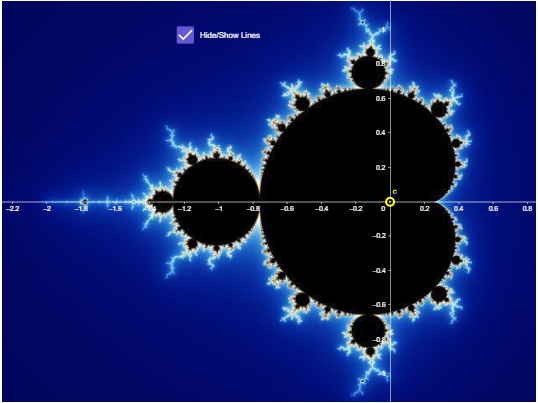
\includegraphics[width=\linewidth]{image9.png}

% \protect\hypertarget{_Toc167901654}{}{}Abbildung 4: Veranschaulichung
% der Folge \(z_{n + 1} = z_{n}^{2}\) mit \(z_{0} = 0\) mittels
% GeoGebra (\url{https://www.geogebra.org/m/Npd3kBKn})

Diese Darstellung lässt vermuten, dass die Folge
\(\left( z_{n} \right)\) für \(z_{0} = 0\) gegen den Wert
\(a = 0\) konvergent ist, da an dieser Stelle ein Häufungspunkt zu
erkennen ist. Diese Vermutung muss nun untersucht werden. Betrachtet man
zunächst die ersten Folgenglieder:

\begin{longtable}[]{@{}
  >{\raggedright\arraybackslash}p{(\columnwidth - 2\tabcolsep) * \real{0.0600}}
  >{\raggedright\arraybackslash}p{(\columnwidth - 2\tabcolsep) * \real{0.9400}}@{}}
\toprule()
\begin{minipage}[b]{\linewidth}\raggedright
\end{minipage} & \begin{minipage}[b]{\linewidth}\raggedright
\[z_{0} = 0\]

\[z_{1} = 0^{2} + 0 = 0 + 0 = 0\]

\[z_{2} = 0^{2} + 0 = 0 + 0 = 0\]

\[z_{3} = 0^{2} + 0 = 0 + 0 = 0\]

...
\end{minipage} \\
\midrule()
\endhead
\bottomrule()
\end{longtable}

Wie anhand der ersten Folgenglieder erkennbar ist, wird nur der Wert 0
angenommen, die Folge konvergiert also gegen 0. Dieses Beispiel ist
trivial und kann somit einen guten Einstieg in die Thematik der
Folgenkonvergenz bieten. Zudem kann so gezeigt werden, dass
„\(\infty\)`` nicht zwingend das letzte Glied einer Folge ist. Außerdem
kann in diesem Zusammenhang thematisiert werden, dass der Grenzwert
erreicht werden kann, aber nicht muss.

\section{Beispiel für Divergenz ($c=-1$)}

Man betrachte die Folge \(\left( z_{n} \right)\) mit der
Bildungsvorschrift \(z_{n + 1} = z_{n}^{2} + c\) mit
\(n \in \mathbb{N}_{0}\) und \(c =  - 1\), der Startwert ist dabei
\(z_{0} =  - 1\). Diese wird mittels eines GeoGebra Applets
veranschaulicht.

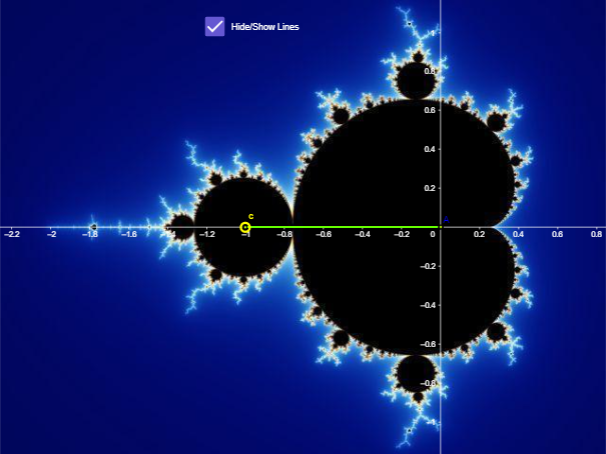
\includegraphics[width=\linewidth]{image10.png}

% \protect\hypertarget{_Toc167901655}{}{}Abbildung 5: Darstellung der
% Folge \(z_{n + 1} = z_{n}^{2}–1\) mit \(z_{0} =  - 1\)
% mittels GeoGebra (\url{https://www.geogebra.org/m/Npd3kBKn})

Diese Darstellung lässt vermuten, dass die Folge
\(\left( z_{n} \right)\) für \(z_{0} =  - 1\) divergent ist, da
sowohl bei \(-\)1 als auch bei 0 ein Häufungspunkt zu erkennen ist. Da
die bildliche Darstellung allein aber nicht ausreicht, muss diese
Vermutung nun genauer untersucht werden. Betrachtet man zunächst die
ersten Folgenglieder:

\begin{longtable}[]{@{}
  >{\raggedright\arraybackslash}p{(\columnwidth - 4\tabcolsep) * \real{0.0561}}
  >{\raggedright\arraybackslash}p{(\columnwidth - 4\tabcolsep) * \real{0.8745}}
  >{\raggedright\arraybackslash}p{(\columnwidth - 4\tabcolsep) * \real{0.0694}}@{}}
\toprule()
\begin{minipage}[b]{\linewidth}\raggedright
\end{minipage} & \begin{minipage}[b]{\linewidth}\raggedright
\[z_{0} =  - 1\]

\[z_{1} = ( - 1)^{2} - 1 = 1 - 1 = 0\]

\[z_{2} = 0^{2} - 1 = 0 - 1 =  - 1\]

\[z_{3} = ( - 1)^{2} - 1 = 1 - 1 = 0\]

\[z_{4} = 0^{2} - 1 = 0 - 1 =  - 1\]

\[z_{5} = ( - 1)^{2} - 1 = 1 - 1 = 0\]

...
\end{minipage} & \begin{minipage}[b]{\linewidth}\raggedright
\end{minipage} \\
\midrule()
\endhead
\bottomrule()
\end{longtable}

Betrachtet man die ersten Folgenglieder, so ist eindeutig erkennbar,
dass die Folge abwechselnd die beiden Werte 0 und \(-\)1 annimmt. Sie
ist somit divergent.

Wie dieses Beispiel zeigt, kann die Mandelbrot-Menge nicht nur zur
Veranschaulichung der Konvergenz, sondern auch zur Visualisierung von
Divergenz eingesetzt werden. Außerdem bietet es sich an, in diesem
Zusammenhang auf Häufungspunkte einzugehen.

\section{Weiteres Beispiel einer Konvergenz ($c=0.25$)}

Ein weniger triviales Beispiel für eine konvergente Folge ist
\(\left( z_{n} \right)\) mit der Bildungsvorschrift
\(z_{n + 1} = z_{n}^{2} + c\) mit \(n \in \mathbb{N}_{0}\) und
\(c = 0.25\), der Startwert ist dabei \(z_{0} = 0.25\). Auch
diese Folge wird mit einem GeoGebra Applet visualisiert.

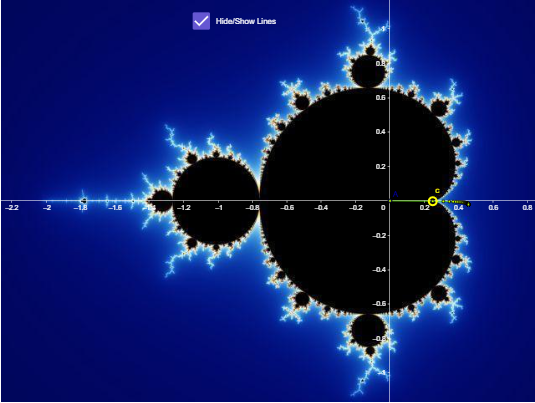
\includegraphics[width=\linewidth]{image11.png}

% \protect\hypertarget{_Toc167901656}{}{}Abbildung 6: Visualisierung der
% Folge \(z_{n + 1} = z_{n}^{2} + 0.25\) mit \(z_{0} = 0.25\)
% mittels GeoGebra (\url{https://www.geogebra.org/m/Npd3kBKn})

Diese Darstellung lässt vermuten, dass die Folge
\(\left( z_{n} \right)\) für \(z_{0} = 0.25\) konvergent ist, auch
wenn der Grenzwert \(a\) nicht direkt abgelesen werden kann.

\begin{longtable}[]{@{}
  >{\raggedright\arraybackslash}p{(\columnwidth - 4\tabcolsep) * \real{0.0236}}
  >{\raggedright\arraybackslash}p{(\columnwidth - 4\tabcolsep) * \real{0.9514}}
  >{\raggedright\arraybackslash}p{(\columnwidth - 4\tabcolsep) * \real{0.0250}}@{}}
\toprule()
\begin{minipage}[b]{\linewidth}\raggedright
\end{minipage} & \begin{minipage}[b]{\linewidth}\raggedright
\textbf{Beweis:}

Betrachtet man zunächst die ersten Folgenglieder:

\[z_{0} = 0.25\]

\[z_{1} = {0.25}^{2} + 0.25 = 0.0625 + 0.25 = 0.3125\]

\[z_{2} = {0.3125}^{2} + 0.25 = 0.3476...\]

\[z_{3} = {0.3476...}^{2} + 0.25 = 0.3708...\]

\[z_{4} = {0.3708...}^{2} + 0.25 = 0.3875...\]

\[z_{5} = {0.3875...}^{2} + 0.25 = 0.4001...\]

\[z_{6} = {0.4001...}^{2} + 0.25 = 0.4101...\]

...

Diese Werte lassen keine eindeutige Vermutung über das Konvergenz- oder
Divergenzverhalten zu, da die Folge monoton steigend zu seien scheint.
Abbildung 6 deutet aber stark auf eine Konvergenz hin.

Daher nehmen wir an, dass die Folge \(\left( z_{n} \right)\) für
\(z_{0} = 0.25\) einen Grenzwert \(a\) besitzt, wenn
\(n \rightarrow \infty\) und versuchen nun, dies zu beweisen.

Wie nehmen an, dass die Folge \(\left( z_{n} \right)\) für
\(z_{0} = 0.25\) einen Grenzwert \(a\) besitzt, wenn
\(n \rightarrow \infty\).

Dann muss gelten:

\[z_{n + 1} = z_{n}^{2} + 0.25\overset{\Leftrightarrow}{\binom{n \rightarrow \infty}{\left( z_{n} \right) \rightarrow a}}a = a^{2} + 0.25 \Longleftrightarrow 0 = a^{2} - a + 0.25\]

Also gilt für den Grenzwert \(a\):

\[a = \frac{1}{2} \pm \sqrt{\left( \frac{1}{2} \right)^{2} - 0.25} = \frac{1 \pm \sqrt{0}}{2} = \frac{1}{2}\]

Das heißt, wir haben den möglichen Grenzwert \(a = 0.5\) der Folge
\(\left( z_{n} \right)\) für \(z_{0} = 0.25\) gefunden (Kovács,
2019, S. 16).

Um zu beweisen, dass \(a = 0.5\) wirklich der Grenzwert der Folge
ist, zeigen wir, dass \(z_{n}\) monoton steigend und von \(a = 0.5\)
beschränkt wird, das heißt, dass \(z_{n} \leq 0.5\) für alle
\(n\mathbb{ \in N}\).

\begin{enumerate}
\def\labelenumi{\arabic{enumi})}
\item
  Monotonie:
\end{enumerate}

\begin{quote}
Induktionsanfang (\(n = 0\)):
\end{quote}

\[z_{0} = 0.25 \leq z_{1} = 0.3125\]

Induktionsschritt:

\begin{quote}
Induktionsannahme: \(\forall n \in \mathbb{N:}z_{n + 1} \geq z_{n}\)

Induktionsbehauptung:
\(\forall n \in \mathbb{N:}z_{n + 2} \geq z_{n + 1}\)
\end{quote}

\[z_{n + 2} = {z_{n + 1}}^{2} + 0.25 \geq z_{n + 1}\]

\begin{quote}
Also ist die Folge \(z_{n}\) monoton steigend.
\end{quote}

\begin{enumerate}
\def\labelenumi{\arabic{enumi})}
\setcounter{enumi}{1}
\item
  Beschränktheit:
\end{enumerate}

\begin{quote}
\(z_{n} \leq 0.5\) für alle \(n\mathbb{ \in N}\)

Induktionsanfang (\(n = 0\)):
\end{quote}

\[z_{0} = 0.25 \leq 0.5\]

Induktionsschritt:

\begin{quote}
Induktionsannahme: \(\forall n \in \mathbb{N:}z_{n} \leq 0.5\)

Induktionsbehauptung:
\(\forall n \in \mathbb{N:}z_{n + 1} \leq 0.5\)
\end{quote}

\[z_{n + 1} = {z_{n}}^{2} + 0.25 \leq {0.5}^{2} + 0.25 \leq 0.5\]

\begin{quote}
Also ist die Folge \(z_{n}\) beschränkt durch 0.5.

Aus der Monotonie und der Beschränktheit der Folge \(z_{n}\) folgt also,
dass \(a = 0.5\) wirklich der Grenzwert der Folge \(z_{n}\) ist.
\end{quote}

\[\blacksquare\]
\end{minipage} & \begin{minipage}[b]{\linewidth}\raggedright
\end{minipage} \\
\midrule()
\endhead
\bottomrule()
\end{longtable}

Eine Visualisierung dieses Beispiels zeigt die Konvergenz besonders
schön, da der Verlauf der Folgenglieder gut zu sehen ist. Die Konvergenz
ist aber nicht trivial und zeigt die Notwendigkeit von Beweisen.

\section{$c=-0.5$ ist Element der Mandelbrot-Menge}

Ein weniger einfaches Beispiel für eine konvergente Folge ist
\(\left( z_{n} \right)\) mit der Regel \(z_{n + 1} = z_{n}^{2} + c\) mit
\(n \in \mathbb{N}_{0}\) und \(c =  - 0.5\), der Startwert ist dabei
\(z_{0} =  - 0.5\). Auch diese Folge kann mit einem GeoGebra Applet
veranschaulicht werden.

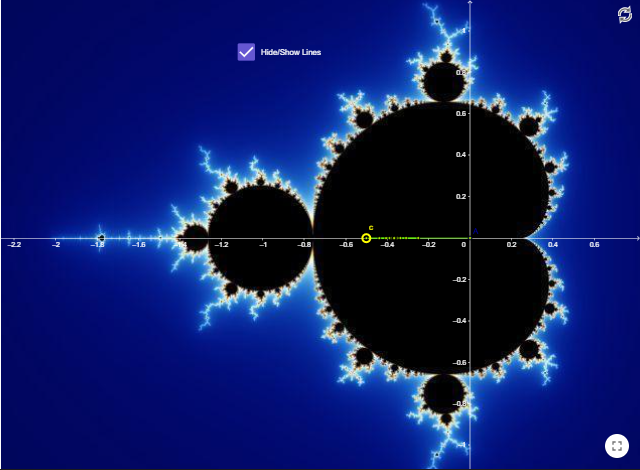
\includegraphics[width=\linewidth]{image12.png}

% \protect\hypertarget{_Toc167901657}{}{}Abbildung 7: Visualisierung der
% Folge \(z_{n + 1} = z_{n}^{2} - 0.5\) mit \(z_{0} =  - 0.5\)
% mittels GeoGebra (\url{https://www.geogebra.org/m/Npd3kBKn})

Diese Abbildung legt die Vermutung nahe, dass die Folge konvergent ist
und der Grenzwert \(a\) zwischen \(-\)0.5 und \(-\)0.25 liegt.

\begin{longtable}[]{@{}
  >{\raggedright\arraybackslash}p{(\columnwidth - 4\tabcolsep) * \real{0.0559}}
  >{\raggedright\arraybackslash}p{(\columnwidth - 4\tabcolsep) * \real{0.8750}}
  >{\raggedright\arraybackslash}p{(\columnwidth - 4\tabcolsep) * \real{0.0691}}@{}}
\toprule()
\begin{minipage}[b]{\linewidth}\raggedright
\end{minipage} & \begin{minipage}[b]{\linewidth}\raggedright
\textbf{Beweis:}

Betrachtet man zunächst die ersten Folgenglieder:

\[z_{0} =  - 0.5\]

\[z_{1} = ( - {0.5)}^{2} - 0.5 = 0.25 - 0.5 =  - 0.25\]

\[z_{2} = ( - {0.25)}^{2} - 0.5 =  - 0.4375\]

\[z_{3} = {( - 0.4375)}^{2} - 0.5 =  - 0.3085...\]

\[z_{4} = {( - 0.3085...)}^{2} - 0.5 =  - 0.4047...\]

\[z_{5} = {( - 0.4047...)}^{2} - 0.5 =  - 0.3361...\]

\[z_{6} = {( - 0.3361...)}^{2} - 0.5 =  - 0.3869...\]

...

Diese Werte liegen zwischen \(-\)0.5 und \(-\)0.25 und scheinen sich
einem Wert zwischen diesen beiden anzunähern, wobei die Werte für
\(n \in \mathbb{N}_{g}\) beginnend bei \(-\)0.5 monoton wachsend
gegen einen Grenzwert und die Werte für \(n \in \mathbb{N}_{u}\)
beginnend bei \(-\)0.25 monoton fallend gegen diesen Grenzwert zu
streben scheinen.

Wie nehmen an, dass die Folge \(\left( z_{n} \right)\) für
\(z_{0} =  - 0.5\) einen Grenzwert \(a\) besitzt, wenn
\(n \rightarrow \infty\).

Dann muss gelten:

\[z_{n + 1} = z_{n}^{2} - 0.5\overset{\Leftrightarrow}{\binom{n \rightarrow \infty}{\left( z_{n} \right) \rightarrow a}}a = a^{2} - 0.5 \Longleftrightarrow 0 = a^{2} - a - 0.5\]

Also gilt für den Grenzwert \(a\):

\[a = \frac{1}{2} \pm \sqrt{\left( \frac{1}{2} \right)^{2} + 0.5} = \frac{1}{2} \pm \sqrt{\frac{3}{4}} = \frac{1 \pm \sqrt{3}}{2}\]

Das heißt, die Fixpunkte der rekursiv definierten Folge und somit die
möglichen Grenzwerte der Folge \(\left( z_{n} \right)\) für
\(z_{0} =  - 0.5\) sind \(a = \frac{1 \pm \sqrt{3}}{2}\).

Nun prüfen wir, ob einer der beiden Fixpunkte wirklich Grenzwert der
Folge ist. Dazu betrachten wir zwei Teilfolgen \(x_{n}\) und \(y_{n}\)
von \(z_{n}\).

Seien \(x_{n}\) und \(y_{n}\) Teilfolgen von \(z_{n}\), wobei
\(n \in \mathbb{N}_{g}\) für \(x_{n}\) und
\(n \in \mathbb{N}_{u}\)für \(y_{n}\).

Betrachten wir die Folge \(x_{n}\).

\[x_{0} = z_{0} =  - 0.5\]

\[x_{1}{= z}_{2} = {z_{1}}^{2} - 0.5 = ({z_{0}}^{2} - 0.5)^{2} - 0.5 = {x_{0}}^{4} - {x_{0}}^{2} - 0.25\]

\[x_{2} = z_{4} = {z_{3}}^{2} - 0.5 = ({z_{2}}^{2} - 0.5)^{2} - 0.5 = {x_{1}}^{4} - {x_{1}}^{2} - 0.25\]

\[x_{3} = z_{6} = {z_{5}}^{2} - 0.5 = ({z_{4}}^{2} - 0.5)^{2} - 0.5 = {x_{2}}^{4} - {x_{2}}^{2} - 0.25\]

...

\[x_{n + 1} = {x_{n}}^{4} - {x_{n}}^{2} - 0.25\]

Um Konvergenz der Folge \(x_{n}\) beweisen zu können, müssen wir zeigen,
dass \(x_{n}\) sowohl beschränkt als auch monoton im Intervall
\(- 0.5{\leq x}_{n} \leq  - 0.25\) ist. Das zeigen wir durch
vollständige Induktion über n.

\begin{quote}
z. z. \(x_{n}\) ist beschränkt und monoton

Induktionsanfang (\(n = 0\)):
\end{quote}

\[- 0.5 \leq  - 0.5 \leq  - 0.25\]

\[{{- 0.4375 = x}_{1} > x}_{0} =  - 0.5\]

\begin{quote}
Induktionsschritt:

Induktionsannahme:
\(\forall n \in \mathbb{N:} - 0.5{\leq x}_{n} \leq  - 0.25\)
und \(x_{n + 1} > x_{n}\)

Induktionsbehauptung:
\(\forall n \in \mathbb{N:} - 0.5{\leq x}_{n + 1} \leq  - 0.25\)
und \(x_{n + 2} > x_{n + 1}\)
\end{quote}

\begin{enumerate}
\def\labelenumi{\arabic{enumi})}
\item
  Monotonie:
\end{enumerate}

\begin{quote}
z.z. für \(- 0.5{\leq x}_{n} \leq  - 0.25\) ist
\(x_{n + 1} > x_{n}\) bzw. \(x_{n + 1} - {x}_{n} > 0\)
\end{quote}

\[f(x) = x^{4} - x^{2} - x - 0.25\]

\begin{quote}
Wir untersuchen nun, wann \(f(x) > 0\) gilt. Hierzu lösen wir die
Ungleichung im Intervall \(- 0.5{\leq x}_{n} \leq  - 0.25\).
\end{quote}

\[f(x) > 0\]

\[x^{4} - x^{2} - x - 0.25 > 0\]

\[4x^{4} - {4x}^{2} - 4x - 1 > 0\]

\[4x^{4} - {4x}^{3} + {4x}^{3} - {2x}^{2} - {4x}^{2} + {2x}^{2} - 2x - 2x - 1 > 0\]

\[2x^{2} \bullet ({2x}^{2} - 2x - 1) + 2x \bullet ({2x}^{2} - 2x - 1) + {2x}^{2} - 2x - 1 > 0\]

\[{(2x}^{2} - 2x - 1) \bullet ({2x}^{2} + 2x + 1) > 0\]

\begin{quote}
Fallunterscheidung:
\end{quote}

\begin{enumerate}
\def\labelenumi{\arabic{enumi}.}
\item
  Fall:
\end{enumerate}

\[{2x}^{2} - 2x - 1 > 0;{2x}^{2} + 2x + 1 > 0\]

\begin{quote}
Wir lösen zunächst die Ungleichung \({2x}^{2} - 2x - 1 > 0\):
\end{quote}

\[{2x}^{2} - 2x - 1 > 0\]

\[{2x}^{2} - 2x - 1 = 0\]

\[x_{1,2} = \frac{1}{2} \pm \sqrt{\left( \frac{1}{2} \right)^{2} + 0.5} = \frac{1}{2} \pm \sqrt{\frac{3}{4}} = \frac{1 \pm \sqrt{3}}{2}\]

\[{2x}^{2} - 2x - 1 = 2 \bullet (x - \frac{1 + \sqrt{3}}{2}) \bullet (x - \frac{1 - \sqrt{3}}{2}) > 0\]

\[(x - \frac{1 + \sqrt{3}}{2}) \bullet (x - \frac{1 - \sqrt{3}}{2}) > 0\]

\[(x - \frac{1 + \sqrt{3}}{2}) > 0 \land (x - \frac{1 - \sqrt{3}}{2}) > 0\]

\begin{quote}
oder
\end{quote}

\[(x - \frac{1 + \sqrt{3}}{2}) < 0 \land (x - \frac{1 - \sqrt{3}}{2}) < 0\]

\begin{quote}
Also:
\end{quote}

\[x > \frac{1 + \sqrt{3}}{2} \land x > \frac{1 - \sqrt{3}}{2}\]

\begin{quote}
oder
\end{quote}

\[x < \frac{1 + \sqrt{3}}{2} \land x < \frac{1 - \sqrt{3}}{2}\]

\begin{quote}
Somit folgt für die Lösungsmenge:
\end{quote}

\[x \in \left\langle  - \infty,\frac{1 - \sqrt{3}}{2} \right\rangle \cup \left\langle \frac{1 + \sqrt{3}}{2},\infty \right\rangle\]

\begin{quote}
Nun betrachten wir noch die zweite Ungleichung des 1. Falls:
\end{quote}

\[{2x}^{2} + 2x + 1 > 0\]

\begin{quote}
Diese Ungleichung ist für alle \(x\mathbb{ \in R}\) erfüllt.

Somit ist die Lösungsmenge für den 1. Fall:
\end{quote}

\[x \in (\left\langle  - \infty,\frac{1 - \sqrt{3}}{2} \right\rangle \cup \left\langle \frac{1 + \sqrt{3}}{2},\infty \right\rangle) \cap x\mathbb{ \in R}\]

\[x \in \left\langle  - \infty,\frac{1 - \sqrt{3}}{2} \right\rangle \cup \left\langle \frac{1 + \sqrt{3}}{2},\infty \right\rangle\]

\begin{enumerate}
\def\labelenumi{\arabic{enumi}.}
\setcounter{enumi}{1}
\item
  Fall:
\end{enumerate}

\[{2x}^{2} - 2x - 1 < 0;{2x}^{2} + 2x + 1 < 0\]

\begin{quote}
Die Berechnungen im 2. Fall sind analog zum ersten Fall. Es ergeben sich
folgende Lösungen:

\({2x}^{2} - 2x - 1 < 0\):
\end{quote}

\[x \in \left\langle \frac{1 - \sqrt{3}}{2},\frac{1 + \sqrt{3}}{2} \right\rangle\]

\begin{quote}
Und für:

\({2x}^{2} + 2x + 1 < 0\):
\end{quote}

\[x \in \varnothing\]

\begin{quote}
Somit insgesamt:
\end{quote}

\[x \in \varnothing\]

\begin{quote}
Die Vereinigung der Lösungsmengen der beiden Fälle ergibt folglich:
\end{quote}

\[x \in \left\langle  - \infty,\frac{1 - \sqrt{3}}{2} \right\rangle \cup \left\langle \frac{1 + \sqrt{3}}{2},\infty \right\rangle\]

\begin{quote}
Somit ergibt sich für das untersuchte Intervall
\(- 0.5{\leq x}_{n} \leq  - 0.25\), dass die Funktion \(f\) im
Intervall
\(\left\langle - 0.5,\frac{1 - \sqrt{3}}{2} \right\rangle\)
monoton steigend ist.
\end{quote}

\begin{enumerate}
\def\labelenumi{\arabic{enumi})}
\setcounter{enumi}{1}
\item
  Beschränktheit:
\end{enumerate}

\begin{quote}
Angenommen \(- 0.5{\leq x}_{n} \leq  - 0.25\) gilt.

Wir betrachten:
\(x_{n + 1} = {x_{n}}^{4} - {x_{n}}^{2} - 0.25\) für
\(x_{n} =  - 0.5\) und \(x_{n} =  - 0.25\) (Intervallgrenzen)

Für \(x_{n} =  - 0.5\):
\(x_{n + 1} = {( - 0.5)}^{4} - {( - 0.5)}^{2} - 0.25 =  - 0,4375\)

Für \(x_{n} =  - 0.25\):
\(x_{n + 1} = {( - 0.25)}^{4} - {( - 0.25)}^{2} - 0.25 =  - 0,3085...\)

Also gilt
\(\forall n \in \mathbb{N:} - 0.5{\leq x}_{n + 1} \leq  - 0.25\),
da die Folge \(x_{n}\) für
\(- 0.5{\leq x}_{n} \leq  - 0.25\) monoton steigend ist und
die Werte \({x}_{n + 1}\) innerhalb von
\(- 0.5{\leq x}_{n + 1} \leq  - 0.25\) liegen.

Insgesamt gilt also für \(x_{n}\), dass die Folge im Intervall
\(- 0.5{\leq x}_{n} \leq  - 0.25\) monoton wachsend und
beschränkt ist. Nach dem Monotonieprinzip (siehe Kapitel 2.1.2) gilt
also, dass \(x_{n}\) konvergiert. Der Grenzwert ist dabei
\(a = \frac{1 - \sqrt{3}}{2}\). Dieser kann aus der Lösung der
Gleichung \(x^{4} - x^{2} - x - 0.25 = 0\) ermittelt
werden.
\end{quote}

Betrachten wir die Folge \(y_{n}\).

\[y_{0} = z_{1} =  - 0.25\]

\[y_{1}{= z}_{3} = {z_{2}}^{2} - 0.5 = ({z_{1}}^{2} - 0.5)^{2} - 0.5 = {y_{0}}^{4} - {y_{0}}^{2} - 0.25\]

\[y_{2} = z_{5} = {z_{4}}^{2} - 0.5 = ({z_{3}}^{2} - 0.5)^{2} - 0.5 = {y_{1}}^{4} - {y_{1}}^{2} - 0.25\]

\[y_{3} = z_{7} = {z_{6}}^{2} - 0.5 = ({z_{6}}^{2} - 0.5)^{2} - 0.5 = {y_{2}}^{4} - {y_{2}}^{2} - 0.25\]

...

\[y_{n + 1} = {y_{n}}^{4} - {y_{n}}^{2} - 0.25\]

Die Konvergenz der Folge \(y_{n}\) im Intervall
\(- 0.5{\leq y}_{n} \leq  - 0.25\) beweisen wir, indem wir,
wie im Fall \(x_{n}\), zeigen, dass \(y_{n}\) sowohl beschränkt als auch
monoton ist. Hier verwenden wir ebenfalls eine vollständige Induktion
über n. Die Schritte dieses Beweises sind hierbei analog zum Beweis für
die Folge \(x_{n}\). Und auch der Grenzwert kann analog, durch lösen der
Gleichung \(y^{4} - y^{2} - y - 0.25 = 0\) ermittelt
werden und ist dabei \(a = \frac{1 - \sqrt{3}}{2}\).

Beide Teilfolgen \(x_{n}\) und \(y_{n}\) von \(z_{n}\) konvergieren also
gegen denselben Wert. Folglich ist die gesamte Folge \(z_{n}\)
konvergent gegen diesen Grenzwert \(a = \frac{1 - \sqrt{3}}{2}\).

\[\blacksquare\]
\end{minipage} & \begin{minipage}[b]{\linewidth}\raggedright
\end{minipage} \\
\midrule()
\endhead
\bottomrule()
\end{longtable}

Dieses Beispiel ist nicht trivial und benötigt für den Beweis ein
tieferes Verständnis der Mathematik und weiterreichende Konzepte als die
bisherigen Beispiele. Ein solches Beispiel kann sich für den Einsatz an
der Universität anbieten.

\section{Noch ein Beispiel einer Divergenz ($c=1$)}

Nicht alle reellen Zahlen sind Element der Mandelbrot-Menge, wie am
Beispiel von \(c = 1\) gezeigt werden kann. Ein weiteres Beispiel
für eine divergente Folge ist \(\left( z_{n} \right)\) mit der
Bildungsvorschrift \(z_{n + 1} = z_{n}^{2} + c\) mit
\(n \in \mathbb{N}_{0}\) und \(c = 1\), der Startwert ist dabei
\(z_{0} = 1\).

\begin{longtable}[]{@{}
  >{\raggedright\arraybackslash}p{(\columnwidth - 4\tabcolsep) * \real{0.0561}}
  >{\raggedright\arraybackslash}p{(\columnwidth - 4\tabcolsep) * \real{0.8747}}
  >{\raggedright\arraybackslash}p{(\columnwidth - 4\tabcolsep) * \real{0.0692}}@{}}
\toprule()
\begin{minipage}[b]{\linewidth}\raggedright
\end{minipage} & \begin{minipage}[b]{\linewidth}\raggedright
\textbf{Beweis:}

Betrachtet man zunächst die ersten Folgenglieder:

\[z_{0} = 1\]

\[z_{1} = 1^{2} + 1 = 1 + 1 = 2\]

\[z_{2} = 2^{2} + 1 = 5\]

\[z_{3} = 5^{2} + 1 = 26\]

\[z_{4} = 26^{2} + 1 = 677\]

\[z_{5} = 677^{2} + 1 = 458330\]

...

Diese Werte deuten stark auf ein divergentes Verhalten der Folge hin.

Wir beweisen die Divergenz über das Minorantenkriterium für Folgen, d.h.
wir betrachten eine Folge \(x_{n}\), die kleiner als \(z_{n}\) ist und
wenn diese Folge divergiert, folgt daraus, dass auch \(z_{n}\) divergent
ist.

Wir betrachten zunächst die Folge \(x_{n + 1} = {x_{n}}^{2}\) mit
\(x_{0} = 2\).

\[x_{0} = 2\]

\[x_{1} = 2^{2} = 4\]

\[x_{2} = 4^{2} = 16\]

\[x_{3} = 16^{2} = 256\]

...

Die Folge \(x_{n}\) kann explizit angegeben werden durch
\(x_{n} = 2^{2^{n}}\).

Nun betrachten wir den Grenzwert der Folge \(x_{n}\):
\(\lim_{n \rightarrow \infty}x_{n} = \lim_{n \rightarrow \infty}2^{2^{n}} = \infty\).
\(x_{n}\) ist also divergent.

Nun vergleichen wir die Folgen \(x_{n}\) und \(z_{n}\). Für die ersten
Folgenglieder gilt, dass \(x_{n} > \) \(z_{n}\). Allerdings hat die
Rekursionsformel von \(z_{n}\) den zusätzlichen Term „+1``, wodurch die
Folge \(z_{n}\) ab einem bestimmten Wert größer als \(x_{n}\) wird, da
\(z_{n}\) schneller wächst. Somit gilt nach dem Minorantenkriterium für
Folgen, dass \(z_{n}\) divergent ist und folglich ist \(c = 1\) kein
Element der Mandelbrot-Menge.

\[\blacksquare\]
\end{minipage} & \begin{minipage}[b]{\linewidth}\raggedright
\end{minipage} \\
\midrule()
\endhead
\bottomrule()
\end{longtable}

Eine Visualisierung dieses Beispiels ist mit dem bisher genutzten
GeoGebra Applet nicht mehr möglich, da die Skalierung in diesem Applet
nicht ausreicht. Allerdings kann der Beweis dennoch durchgeführt werden.
Auch dieses Beispiel eignet sich für die Universität, da Beweismethoden
und Konzepte verwendet werden, die nicht unbedingt der Schulmathematik
entsprechen. Zudem können Grenzen der Visualisierung thematisiert
werden.


\chapter{Literaturverzeichnis}\label{literaturverzeichnis}

Ableitinger, C., Götz, S. \& Steinbauer, R. (2022). Vorstellungen von

\begin{quote}
Lehramtsstudierenden zum Grenzwertbegriff. \emph{Mathematica Didactica},
45, 1-21.
\end{quote}

Amrhein, B. \& Gloor, O. (1992). Illustrierte Mathematik ---
Visualisierung von

\begin{quote}
mathematischen Gegenständen. In K. Dette, D. Haupt, C. Polze (Hrsg.),
\emph{Multimedia und Computeranwendungen in der Lehre. Reihe
Mikrocomputer-Forum für Bildung und Wissenschaft}, Bd. 5. Springer.
\url{https://doi.org/10.1007/978-3-662-00998-7_39}
\end{quote}

Arens, T., Hettlich, F., Karpfinger, C., Kockelkorn, U., Lichtenegger,
K. \& Stachel, H.

\begin{quote}
(2008). \emph{Mathematik}. Spektrum Akademischer.
\end{quote}

Barnsley, M. (1995). \emph{Fraktale: Theorie und Praxis der
Deterministischen Geometrie}.

\begin{quote}
Spektrum Akademischer.
\end{quote}

Bender, P. (1991). Fehlvorstellungen und Fehlverständnisse bei Folgen
und

\begin{quote}
Grenzwerten. \emph{Der mathematische und naturwissenschaftliche
Unterricht}, 44, 238 - 243.
\end{quote}

Büchter, A., Glade, M., Herold-Blasius, R., Klinger, M., Schacht, F. \&
Scherer, P.

\begin{quote}
(Hrsg.). (2019). \emph{Vielfältige Zugänge zum Mathematikunterricht:
Konzepte und Beispiele aus Forschung und Praxis}. Springer Spektrum.
\end{quote}

Giaquinto, M. (2007). \emph{Visual thinking in mathematics}. Oxford
University Press Inc.

\begin{quote}
\url{https://doi.org/10.1093/acprof:oso/9780199285945.001.0001}
\end{quote}

Greefrath, G., Oldenburg, R., Siller, H., Ulm, V. \& Weigand, H. (2016).
\emph{Didaktik der}

\begin{quote}
\emph{Analysis: Aspekte und Grundvorstellungen zentraler Begriffe}.
Springer Spektrum.
\end{quote}

Hinrichs, A. (2022). \emph{Analysis I für Lehramt - WS 2022/23,
Vorlesungsnotizen von Prof.}

\begin{quote}
\emph{Aicke Hinrichs, mit Überarbeitungen von Markus Passenbrunner.}
(Vorlesungsskript). Johannes-Kepler-Universität Linz.
\end{quote}

Hoch, T. \& Küveler, G. (2023). \emph{C/C++ anwenden} (2. Aufl. überarb.
Aufl.). Springer.

\begin{quote}
\url{https://doi.org/10.1007/978-3-658-38093-9}
\end{quote}

Kovács, Z. (2019). \emph{Teaching fractals for gifted learners at age 12
by using novel}

\begin{quote}
\emph{technologies}. arXiv (Cornell University). Abgerufen von
\url{https://arxiv.org/pdf/1912.08703.pdf}
\end{quote}

Kriz, J. (1992). \emph{Grundkonzepte der Systemtheorie: Chaos und
Struktur, Band 1, mit}

\begin{quote}
\emph{einem Vorw. von Hermann Haken}. Quintessenz.
\end{quote}

Lindenbauer, E., Lindner, A., Schoberleitner, F. (2023).
\emph{Schulmathematik}

\begin{quote}
\emph{Analysis - 2023 S}. (Lehrveranstaltungsskript). Pädagogische
Hochschule OÖ.
\end{quote}

Lucht, P., Schmidt, L. \& Tuma, R. (Hrsg.). (2013). \emph{Visuelles
Wissen und Bilder des}

\begin{quote}
\emph{Sozialen: Aktuelle Entwicklungen in der visuellen Soziologie}.
Springer.
\end{quote}

Mandelbrot, B. (1991). \emph{Die fraktale Geometrie der Natur}.
Birkhäuser.

Mandelbrot, B. (2004). \emph{Fractals and chaos: The Mandelbrot Set and
Beyond}. Springer.

Neunzert, H. (Hrsg.). (1980). \emph{Analysis 1: Ein Lehr- und
Arbeitsbuch für Studienanfänger}.

\begin{quote}
Springer.
\end{quote}

Ostsieker, L. (2020). \emph{Lernumgebungen für Studierende zur
Nacherfindung des}

\begin{quote}
\emph{Konvergenzbegriffs: Gestaltung und empirische Untersuchung}
(Dissertation). Springer Spektrum.
\end{quote}

Peitgen, H. \& Richter, P. H. (1986). \emph{The beauty of fractals:
Images of complex}

\begin{quote}
\emph{dynamical systems}. Springer.
\end{quote}

Phillips, L. M., Norris, S. R. \& Macnab, J. S. (2010).
\emph{Visualization in mathematics,}

\begin{quote}
\emph{reading and science education models in modeling in science
education} (Vol. 5). Springer.
\end{quote}

Precht, M., Voit, K. \& Kraft, R. (1991). \emph{Mathematik 2 für
Nichtmathematiker: Funktionen}

\begin{quote}
\emph{Folgen und Reihen Differential und Integralrechnung
Differentialgleichungen Ordnung und Chaos} (4. Aufl.). Oldenbourg.
\end{quote}

Schmitz, A. (2017). Visualisierung in Mathematik und Mathematikdidaktik.
In A. Schmitz

\begin{quote}
(Hrsg.), \emph{Beliefs von Lehrerinnen und Lehrern der Sekundarstufen
zum Visualisieren im Mathematikunterricht. Freiburger Empirische
Forschung in der Mathematikdidaktik}. Springer Spektrum.
\end{quote}

Sieber, N., Sebastian, H.-J. \& Zeidler, G. (1988). \emph{Mathematik für
Ingenieure,}

\begin{quote}
\emph{Naturwissenschaftler, Ökonomen und Landwirte. Band 1: Grundlagen
der Mathematik, Abbildungen, Funktionen, Folgen} (8. Aufl.) BSB Teubner.
\end{quote}

Walter, W. (1990). \emph{Analysis 1} (2. Aufl.). Springer.

Weigand, H. (2016). Zur Entwicklung des Grenzwertbegriffs unter
stoffdidaktischer

\begin{quote}
Perspektive. \emph{Mathematische Semesterberichte}, 63(1), 135--154.
\url{https://doi.org/10.1007/s00591-016-0161-4}
\end{quote}

Weitz, E. (2018). \emph{Konkrete Mathematik (nicht nur) für
Informatiker}. Springer.

\begin{quote}
\url{https://doi.org/10.1007/978-3-658-21565-1}
\end{quote}

Xaos-Project. (n.~d.). \emph{GitHub - xaos-project/XaoS: Real-time
interactive fractal zoomer}.

\begin{quote}
\url{https://github.com/xaos-project/XaoS} {[}23.03.2024{]}
\end{quote}

\section{Abbildungsverzeichnis}\label{abbildungsverzeichnis}

\protect\hyperlink{_Toc167901651}{Abbildung 1: Mandelbrot-Menge (Hoch \&
Küveler, 2023, S. 163) \protect\hyperlink{_Toc167901651}{13}}

\protect\hyperlink{_Toc167901652}{Abbildung 2: Mandelbrot-Menge in XaoS
(Xaos-Project, n. d.) \protect\hyperlink{_Toc167901652}{22}}

\protect\hyperlink{_Toc167901653}{Abbildung 3: Visualisierung der
Konvergenz für einen bestimmten Wert c in der Mandelbrot-Menge mittels
GeoGebra Applet (https://www.geogebra.org/m/Npd3kBKn)
\protect\hyperlink{_Toc167901653}{23}}

\protect\hyperlink{_Toc167901654}{Abbildung 4: Veranschaulichung der
Folge \(z_{n + 1} = z_{n}^{2}\) mit \(z_{0} = 0\) mittels
GeoGebra (https://www.geogebra.org/m/Npd3kBKn)
\protect\hyperlink{_Toc167901654}{24}}

\protect\hyperlink{_Toc167901655}{Abbildung 5: Darstellung der Folge
\(z_{n + 1} = z_{n}^{2}–1\) mit \({z}_{0} =  - 1\) mittels
GeoGebra (https://www.geogebra.org/m/Npd3kBKn)
\protect\hyperlink{_Toc167901655}{25}}

\protect\hyperlink{_Toc167901656}{Abbildung 6: Visualisierung der Folge
\(z_{n + 1} = z_{n}^{2} + 0.25\) mit \(z_{0} = 0.25\)
mittels GeoGebra (https://www.geogebra.org/m/Npd3kBKn)
\protect\hyperlink{_Toc167901656}{26}}

\protect\hyperlink{_Toc167901657}{Abbildung 7: Visualisierung der Folge
\(z_{n + 1} = z_{n}^{2} - 0.5\) mit \(z_{0} =  - 0.5\)
mittels GeoGebra (https://www.geogebra.org/m/Npd3kBKn)
\protect\hyperlink{_Toc167901657}{29}}

\end{document}
